\chapter{Multimedia Information Retrieval and Indexing}
\label{state1}
	
	The Information Retrieval aims to define approaches and techniques to model, store and 
	access information items \citep{Baeza-Yates2011}.
	The information can take different forms: textual document, an audio sequence, a visual 
	data (images) or a video clip. Thus, the multimedia information retrieval 
	field engages many research areas as signal processing, 
	machine learning, data mining, information theory, human-computer interaction and many other 
	areas \citep{Rueger2010,Sheu2010}. Many researches \revAnglais{have} addressed an important interest to multimedia 
	information retrieval in recent years. In fact, the raising of advanced multimedia devices 
	together with the low cost storage devices have blown-up the production and the 
	access to multimedia data content.

	The present chapter describes basic concepts of multimedia retrieval and indexing which consist of the 
	general architecture and the evolution of retrieval approaches from the text-based toward the concept-based 
	approach. This chapter ends with an enumeration of open issues in semantic video indexing.

	\section{Multimedia Information}

	%In figure \ref{state_fig1}, the information side contains a large amount of multimedia content that the 
	%Information System has to process, analyze and manage. 
	The multimedia content formats can vary 
	according to the usage domain, for example web pages, video sequences, audio sequences, \dots{}. 
	All these broadly different \revAnglais{understandings} of what a multimedia content \revAnglais{help} to interpret the 
	semantics within a defined content. In fact, for a given multimedia content, we can identify different
	basic data types (such as text, image, video, speech, audio), interactive elements 
	(links, event on user action, mouse over, \dots{}) and structural elements (text formatting, image and 
	video location, \dots{}). The syntax of a multimedia content is a collection of several different  data 
	types that provide rich information and enhanced experience for the reader \citep{Stamou2005}.

	As depicted in figures \ref{state_fig2} and  \ref{state_fig3}, we conclude that humans segment a multimedia 
	document into manageable blocks of information in order to construct a complete understanding of 
	that content. Thus, in this thesis, we consider a multimedia content as an image and audio stream 
	that carry some semantic information. The figure \ref{state_fig3} illustrates a scene of car racing. 
	While the first segment depicts some racing cars, the second segment depicts aligned cars at the start 
	line. By identifying valuable objects and sounds within that content, we aim to generate a more 
	complete and enhanced semantic interpretation. Video segmentation, visual objects detection and audio 
	analysis are discussed in two other thesis works \citep{Feki2013,Elleuch2015a} 
	carried out jointly with the present one.

	\begin{figure}[ht]
		\centering
		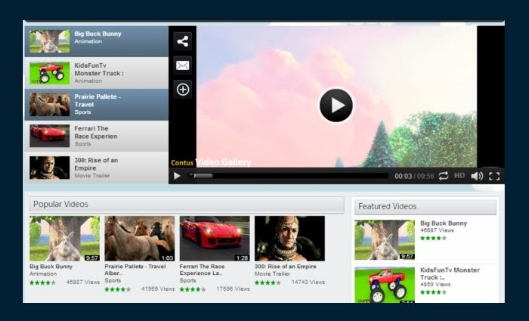
\includegraphics[scale=0.8]{figures/state_fig3}
		\caption{A Web page can be seen as a multimedia document}
		\label{state_fig2}
	\end{figure}

	\begin{figure}[ht]
		\centering
		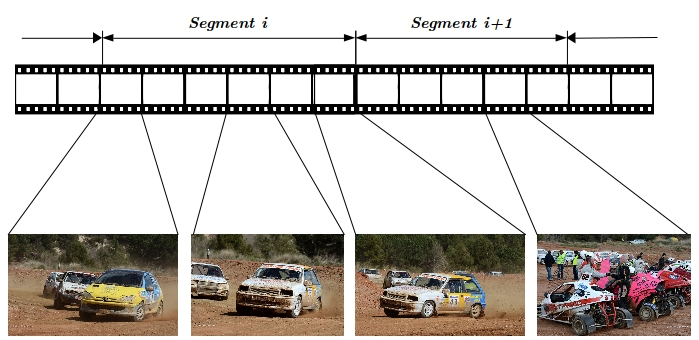
\includegraphics[scale=0.7]{figures/state_fig4}
		\caption{Video sequences can be seen as a multimedia document}
		\label{state_fig3}
	\end{figure}

	%In the figure \ref{state_fig1}, the user side displays a generic paradigm of Information retrieval: 
	%the user defines some information need, and the system supplies the required information. 

	Unlike textual documents, a multimedia content contains more than symbols that a user can take on 
	in order to express his need for information. At first, the multimedia content is rich in term 
	of available semantic information: the visual content can expose a variety of messages and emotions, 
	an audio content can also expose feeling and emotions, then, the structure itself 
	(spatial-temporal information) also communicates valuable information. Thus, a multimedia content 
	delivers a complete semantic interpretation to be communicated to the user. Secondly, the computational 
	system can process only mathematical and logic expressions, and not all what a human can express 
	and interpret in term of ideas, emotions and feeling: the communication gap between the user and the system.

	Many approaches were proposed in literature in order to empower the user with tools to express 
	his query and achieve a better mapping between the expressed user need, the extracted 
	multimedia information, and what the system can  successfully match. Some of these techniques 
	will be exposed in the following sections.

	\section{Multimedia Information Retrieval}

	In order to access a multimedia content, some techniques are used to interpret a
	human queries that translate its needs, and then to retrieve the closest match. 
	As an example, a user searches its collection using the keyword or a phrase such 
	as \emph{car} or \emph{car racing}, he will expect the information retrieval system 
	to return all relevant items. Nevertheless, the user still disappointed with the given 
	results. Such a disappointment can be rooted in two reasons. Firstly, the context in 
	which the user has expressed its information need could be too vague and requires the user
	to further refine its query. Secondly, the weak and blurred link between the information
	representation schemes and the user semantic query. These two issues are called the
	\emph{semantic gap} \citep{Smeulders2000,Bahmanyar2015}.

	Low-level extraction approaches from visual contents (e.g., histograms, shapes, motions, \dots)
	and audio content (e.g. volume, frequency, pitch, …) are widely investigated, providing a wide 
	feature sets that could be explored for indexing and modeling a multimedia content. These low-level 
	features rely on data-driven properties and characteristics, which may be misrelated to the concepts 
	expressed in the semantic query.

	The semantic information extraction process from multimedia contents is considered as an artificial 
	intelligence problem. Nevertheless, Human perception is still being not well understood for imitating 
	it in a computational system. In fact, an Information Retrieval (IR) system \revAnglais{is} considered as an 
	artificial intelligence problem, on one hand, because the system has to mimic the human perception 
	process in order to extract relevant semantics from a given multimedia content, and on the other hand, 
	the system has to interpret the user query and match the relevant stored information. 
	Then, the missing relationship between low-level features and human knowledge is the fundamental semantic 
	gap problem when we need to search a multimedia collection by expressing some semantic queries. 
	
	Recent proposed multimedia analysis and indexing approaches rely mainly on manual annotations 
	\citep{Wang2011,Lazaridis2013,Jin2015}. Such approaches are flawed and costly, and can lead to 
	a poor learning process.  As depicted in figure \ref{state_fig1}, the user query is analyzed by the information 
	retrieval system with the same system that can imitate human perception in order to process the query 
	and match it to relevant information. The semantic gap exists in both: (1) multimedia content analysis, 
	and (2) user query understanding.

	In this scope, actual researches in multimedia retrieval are exploring new paradigms for semantic 
	multimedia information analysis in order to deliver a higher degree for semantic information 
	processing capabilities. In fact, the multimedia community addressed more intention on knowledge 
	management based approaches for such a propose. 

	\begin{figure}[ht!]
		\centering
		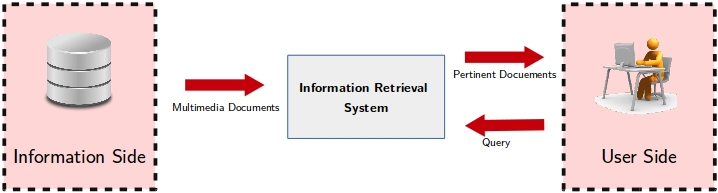
\includegraphics[scale=0.8]{figures/state_fig1}
		\caption{Information work-flow in Information Retrieval}
		\label{state_fig1}
	\end{figure}

	%Before discussing the ontology based approaches,
	We will continue, in the following, 
	to display and identify the information retrieval main research directions. 

	The information system has been proposed since several decades. Most of proposed systems
	until mid $90^{s}$ handled only text data based documents \citep{Manning2008,Marcia2012}.
	 From such an experience, a set of functional components were \revAnglais{defined:}
	(1) the analysis component that extracts a vocabulary from documents, 
	(2) The indexing module that represents documents through its information symbols, 
	(3) the query processing component that transforms a user information needs into information symbols, and 
	(4) the retrieval component that ranks the stored documents representation according to the similarity 
	measure between information symbols.

	A multimedia information system, as displayed in figure \ref{state_fig4}, is similar to the traditional 
	Information retrieval system detailed above, but with different algorithms: the multimedia analysis handles 
	multimedia content unlike a text document. Thus, the information retrieval system architecture depicted in 
	figure \ref{state_fig4} can be addressed as a generic information retrieval system. In the \revAnglais{following}, we detail 
	the components of this generic architecture.

	\begin{figure}[ht]
		\centering
		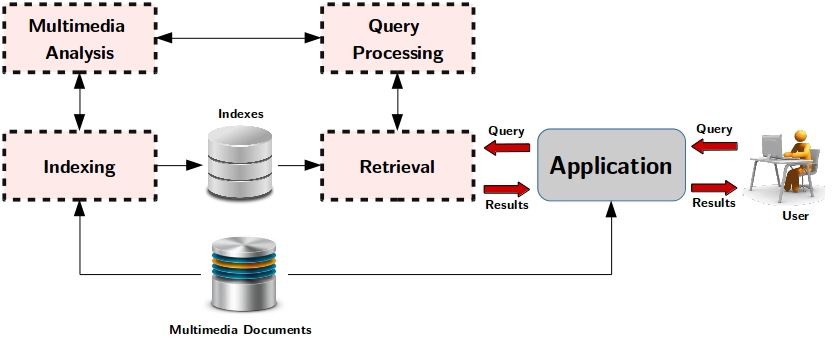
\includegraphics[scale=0.7]{figures/state_fig2}
		\caption{Classic Multimedia Information Retrieval Architecture}
		\label{state_fig4}
	\end{figure}

		\subsection{Multimedia Analysis}	

		Information Retrieval systems \revAnglais{analyze} multimedia contents and extract features measuring 
		the importance of information symbols. The extraction of these features aims: 
		(1) to associate multimedia contents to meaningful symbols of information that 
		a user can use to search for, and (2) to quickly find relevant document through
		information symbols indexing.

		These information symbols re-extracted automatically, semi-automatically or manually 
		\citep{Zhang2012}. While the automatic information symbols extraction executes an analysis 
		task without a human intervention, the semi-automatic one includes a human as part of the analysis
		task: some information can only be detected and added by a human, such as the name of a person, 
		or the relation between two persons (e.g. friends). Many approaches were proposed, but more adequate
		to the considered information domain. As an example, \textsc{Google} \citep{Chen2011,Kumar2014}
		and \textsc{Flickr} \citep{Sigurbjoernsson2008,Ginsca2014} page rank rely on some human
		intervention in order to edit information, and then improve search results. While \textsc{Flickr} 
		allows the user to tag images with a set of keywords that can be used later for searching images, 
		\textsc{Google} \revAnglais{relies} on human edited links pointing to analyzed web pages in order to adjust its 
		importance. We conclude that \textsc{Flickr} adopts a semi-automatic approach, and \textsc{Google}
		adopts an automatic one since it relies on stored information.

		\begin{figure}[ht]
			\centering
			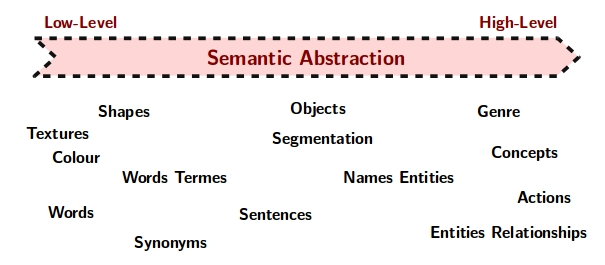
\includegraphics[scale=0.7]{figures/state_fig5}
			\caption{Relation between information symbols and semantic abstraction}
			\label{state_fig5}
		\end{figure}

		The figure \ref{state_fig5} displays some feature \revAnglais{positions on} a semantic abstraction level: 
		from low-level features to high-level ones.  While low-level features, such as color histogram,
		are easily extracted from a multimedia content through automatic methods, high-level features, 
		such as content topic or objects existing in the content, require more complex approaches
		due to the high semantic dimension that they involve.

		Classical text analysis approaches produced a small set of features (e.g. occurring words). 
		However, multimedia analysis approaches generate scores, such as a probability, for all 
		possible features (information symbols). Such a situation will induce to produce dense 
		high-dimensional vectors that contain all features extracted from all multimedia documents, 
		and then cause several issues such as storage space. Thereby, the multimedia analysis approaches
		\revAnglais{are} important since they will impact the entire multimedia \revAnglais{information} system. 
		So, many techniques and algorithms are provided to \revAnglais{dress} these issues.
		
		\begin{itemize}
			\item \textit{Low-Level Analysis: }
				The low-level analysis extracts features from a multimedia content. 
				These features are commonly related to human senses or language (e.g. image colors,
				image textures, audio rhythms, word, \dots{}). Such features are well studied in
				literature and most of them have been developed in the area of data compression 
				that exploits the characteristics of human vision and hearing senses 
				\citep{Foerstner1994,Nixon2012}. 

				These low-level features are used then to index multimedia contents.

			\item \textit{High-Level Analysis: }
				The High-level analysis aims to extract inferred information from a multimedia content. 
				\revAnglais{This} extracted information can be not explicitly detectable by a computer. 
				Then, a prior-knowledge about the problem domain semantics should be involved. 
				Such domain centered knowledge \revAnglais{is} formally described by a set of semantic concepts
				identified by keywords. The latter capture part of domain knowledge which can be used
				to detect the presence of a concept in a given multimedia content. 

				The high-level features (concept/keyword) are used as index tokens that the 
				information retrieval system uses to build the index of a semantic-multimedia content.
		\end{itemize}

		\subsection{Indexing}

		Information features (symbols) extracted from a multimedia content  are stored by the indexing
		component. While the analysis component impacts the effectiveness of the multimedia information 
		system, the indexing one impacts the efficiency of the system. The main aim of the indexing algorithm 
		is to manipulate an inverted-file index that enumerates all information symbols and all 
		related documents that \revAnglais{contain} these symbols.

		The indexing component uses a high-dimensional index to accommodate the high-dimensional 
		multimedia content data nature (as the multimedia analysis component produces a score for 
		all possible feature type and dimension). The efficiency of high-dimensional indexes \revAnglais{is} 
		related to several aspects \citep{Ai2013}: tree-structured indexes, hash-based indexes, compression of the
		index to reduce memory usage,  \dots{}. All these techniques allow a \revAnglais{more} faster and efficient
		look-up of the index table. In \citep{Baeza-Yates1999,Baeza-Yates2011}, the authors discussed 
		the efficiency of the indexing component.


		\subsection{Query Processing}

		When the user communicates query to the information retrieval system, the latter analyses and 
		transforms the query into an internal representation that used the same symbols for indexing
		multimedia contents. 

		The query processing component parses the user query according to a specific language,
		extracts information symbols and features, and proceeds it to the retrieval component 
		to search index for the matching documents.
		
		Text based information retrieval systems \revAnglais{handle} text queries as a query language support. 
		In multimedia information systems, the queries can be expressed in many ways \citep{Liu2007,Yasmin2014}. 
		In what follows, a brief enumeration of some of these queries methods.
		
		\begin{itemize}
			\item \textit{Sketch Retrieval:} this is one of the first proposed methods to query 
			a multimedia database \citep{Cao2010,Cao2011}. The user query is in the form of a visual
			sketch of what the user \revAnglais{expects} to find. The information retrieval system proceeds then the 
			extraction of features from that sketch in order to search the index for images that are 
			visually similar.
			
			\item \textit{Search by Example:} the user can submit an example image representing the 
			information he \revAnglais{is} searching for. In such a case, the query processing extracts the low-level 
			features for the query in order to look for similar stored documents with similar features.
			
			\item \textit{Search by Keyword:} this is by far the most popular search query method: 
			the user describes his information request with a set of keywords. \revAnglais{Then}, the system
			searches for multimedia content that corresponds to these keywords. The issue of this 
			high-level query method is that the user can only use some predefined keyword vocabulary 
			used also in multimedia content indexes.
			
			\item \textit{Personalized/Adaptive Retrieval:} this is a refinement to all other search methods. 
			It explores the history and profile of the user search \citep{Magalhaes2004}. 
			\revAnglais{This} extra-information can enhance the search experience by filtering information
			to particular domains, limiting certain document formats, \dots{}.

		\end{itemize}

		\subsection{Retrieval}

		The retrieval component computes indexed document ranks according to their similarities to a user query. 
		This component browses and sweeps the index according to the input query information symbols to 
		search for most similar documents according to the relevance degree. The latter is computed by a 
		function that determines the semantic relatedness degree between the query and the retrieved documents. 
		Thus, the result delivered by the retrieval component is a set of ordered documents that \revAnglais{are} judged 
		as similar documents to the given query \citep{Memar2013}. 

		The challenging problem in the ranking task is to find which documents are relevant and which
		are irrelevant. The relevance degree between the document and the user query is computed through
		various retrieval models. The information retrieval community proposed different retrieval models
		\citep{Baeza-Yates1999,Croft2010} such as: Boolean, vectorial, probabilistic and fuzzy models.

		\begin{itemize}
			\item \textit{Boolean Model:} is the oldest and the classical retrieval model. 
			It is based on the Boolean algebra. With such a model, a query is defined 
			as a Boolean expression, and the relevance of a document  to a query is computed by the 
			use of Boolean operators like \emph{And}, \emph{NOT} and \emph{OR}. One limitation of 
			the boolean model is that computed relevance weights are equal for all relevant documents: 
			it will be difficult then to identify the most relevant documents between the less ones.
	
			\item \textit{Vector Space Model:} is the most popular and used retrieval model. 
			Both queries and documents are handled as vectors in the space. Then, the 
			similarity between a query and a document is estimated by the use of direction 
			and distance \citep{Manning2008}. 

			\item \textit{Probabilistic Model:} is a model that ranks document according to the 
			probability of relevance to a given query. This model uses the probability ranking 
			principal detailed in \citep{Fuhr1992}. Thus, a statistical distribution is used in order 
			to measure the relevancy between relevant documents and irrelevant ones.

			\item \textit{Fuzzy model: } Fuzzy logic plays an important role in many domains that handle 
			imprecise and vague information \citep{Mantaras2015}, such as text-mining, multimedia 
			information system, machine learning, \dots{}. To handle uncertain information, 
			the fuzzy logic allows intermediate truth values to be defined between 
			conventional evaluations of true (1) and false (0). Fuzzy logic was used as a fuzzy 
			retrieval model \citep{Tahani1976,Cross1994,Miyamoto2012}.
		\end{itemize}

	\section{Multimedia Retrieval Systems Evaluation}
		Information Retrieval has been widely addressed in research work, and it has been shown  
		to be highly useful to compare different systems and approaches. In literature, two different 
		measures are used: Firstly, an effectiveness metric is used to measure how well the system
		can satisfy the user information need. Secondly, the efficiency metrics measures both, 
		the system  responsiveness to the user query, and the system ability to cope with large-scale situations.
		
		Effectiveness and efficiency measures are widely affected by the data that is used to test a system. 
		In fact, a dataset can contain information with different complexities. Therefore, evaluation 
		methodologies are now being investigated and standardized. In the following, we enumerate 
		traditional metrics and resources used in the evaluation of information retrieval systems.

		\subsection{Effectiveness Evaluation}
		In order to introduce the retrieval effectiveness measure, we discuss the meaning of relevance.
		The relevance is a fundamental concept of information retrieval. The paper \citep{Mizzaro1997}
		is considered as the first work that focused on the relevance concept: \emph{the relevance is 
		claimed as a complex concept involving different aspects: methodological foundations, different 
		types of relevance, beyond-topical criteria adopted by users, modes of expression of the relevance 
		judgment, dynamic nature of relevance, types of document representation, and agreement among 
		different judges}.

		Therefore, many research areas adopt their own definition of relevance focusing more \revAnglais{on} their 
		specific objectives: the information retrieval aims to identify documents that can be judged as  
		the best answer to a given information query. Information retrieval relies on document datasets 
		where their relevance of a given query was judged by a human. Nevertheless, there is no general 
		definition of what a relevant document is. In fact, the relevance of  document is a diffuse 
		information because a given document can have different meanings to different humans. 
		This issue was widely discussed in literature that noticed a divergence between relevance 
		judgment made by different human for a given document \citep{Voorhees2000,Volkmer2007}.
		This divergence is more observable in large multimedia datasets. In fact, a multimedia content 
		is by nature subject of different interpretations and relevance annotation (judgment), also, 
		human relevance judgment process is a very costly task and large-scale document datasets will
		be partially annotated (incomplete and inconsistent).

		\emph{Precision} and \emph{recall} \citep{Buckland1994} are the popular information retrieval metrics. They are applied 
		on a ranked list of both relevant and non-relevant documents for a given query. While the precision 
		addresses the accuracy of the evaluated system, the recall addresses the completeness aspect.
		We enumerate, in the following, these two metrics and other derived ones.

		\begin{itemize}
			\item \textit{\textbf{Precision (Prec):}} which measures the ability of a
			system to present only relevant items. Mathematically, the Precision (\emph{Prec})
			is defined as the number of true positive documents ($T_{p}$) over the number of 
			true positives plus the number of false positives ($F_{p}$).
			\begin{equation}
				Prec = \frac{T_{p}}{T_{p} + F_{p}}
			\end{equation}

			\item \textit{\textbf{Recall (Rec):}} which measures the ability of a system
			to present all relevant documents.  Mathematically, the Recall (\emph{Rec}) is defined 
			as the number of true \revAnglais{positive documents} ($T_{p}$) over the number of true positives 
			plus the number of false \revAnglais{negative} documents($F_{n}$).
			\begin{equation}
				Rec =  \frac{T_{p}}{T_{p} + F_{n}}
			\end{equation}

			\item \textit{\textbf{F-measure (Harmonic mean):}} is a measure which assesses the
			trade-off between precision and recall. The \emph{F-measure} is computed as follows:
			\begin{equation}
				F =  \frac{2}{\frac{1}{Prec} + \frac{1}{Rec}}
			\end{equation}

			\item \textit{\textbf{Average Precision (AP):}} is obtained after each relevant 
			document is retrieved. Let $k$  be the number of relevant retrieved documents, the average 
			precision expression is:
			\begin{equation}
				AP = \frac{\sum\limits_{k\in \{r|r \text{ is rank of relevant docs}\}} 
					Prec@k}{\text{Number of relevant Documents}}
			\end{equation}

			\item \textit{\textbf{Mean Average Precision (MAP):}} is a metric which summarizes the
			overall system retrieval effectiveness into a single value as the mean of all 
			keywords average precision,
			\begin{equation}	
				MAP =  \frac{1}{|Q|} \sum_{q \in Q} AP_{q} \text{~~~~~where $Q$ is a set of queries}
			\end{equation}
		\end{itemize}
		These metrics measure the effectiveness of a given system in  fixed evaluation scenario. 
		Thus, the obtained measures are valid only for a specific scenario and \revAnglais{cannot} be generalized 
		to other situations.			

		\subsection{Efficiency Evaluation}

		The efficiency measurement in multimedia information system concerns the extra computational
		complexity over conventional information retrieval systems. This extra complexity is due to 
		the extra processing required to analyze a multimedia content and extract the contained 
		semantics.

		In the context of our thesis, we solely focus on the runtime complexity of the analysis component. 
		In fact, and as discussed in previous sections, the information indexing involves the indexing and 
		the storage of extracted low-level and high level features. The efficiency of the indexing task 
		measures both:
		\begin{itemize}
			\item \textit{Time complexity:} which measures how many documents/concepts per second 
			can the indexing task processes. Thus, the time complexity measures the system responsiveness.

			\item \textit{Space complexity:} which measures the amount of memory required to process a document 
			for the entire vocabulary. The space complexity measures the scalability aspect.
		\end{itemize}
		These two complexities define how well a system scales with several simultaneous requests.


		\subsection{Collections}

		In the assessment of semantic multimedia retrieval systems, multimedia collections 
		are used as research tools that provide a common test environment in order to evaluate and 
		compare different approaches and techniques. 

		Collections are used to evaluate a variety of techniques, such as shot-boundary detection, 
		low-level visual features, story segmentation, \dots{}. In this thesis, we address the problem of 
		indexing multimedia content by their semantic content. One aspect is required to be present in a 
		collection that will be used for the assessment of multimedia indexing: keywords that correspond 
		to concepts present in the collection content. They describe what meaningful concepts are present 
		within a given multimedia content.
	
		Multiple benchmarking initiatives have been proposed which aim the assessment of multimedia 
		retrieval system performances with \revAnglais{standardized} test collections and tasks, such as in 
		\textsc{ImageClef} \citep{Villegas2013,Villegas2014,Villegas2015} and \textsc{TrecVid} 
		\citep{Smeaton2006,Over2013,Over2014}. In what follows, we \revAnglais{enumerate} the multimedia 
		collections/benchmarks addressed in this thesis work.

		\begin{enumerate}
			\item \textit{\textbf{\textsc{ImageClef:}}} \textsc{ImageClef} is an evaluation forum for the 
			cross-language image retrieval.  The main goal of that benchmark is to provide the 
			required infrastructure for the evaluation of visual information retrieval systems 
			operating in monolingual, cross-language and language-independent contexts. 
			Thus, \textsc{ImageClef} allows  multilingual users accessing the growing visual 
			multimedia data, and creates a public resources for benchmarking information retrieval 
			systems and approaches. 

			Since its start in 2003, \textsc{ImageClef} \revAnglais{has been}
			a track in the \emph{Cross Language Evaluation Forum} 
			(\textsc{Clef}). The latter is one of the major forums for research in information retrieval. 
			The main goal is to create collections and topics in order to offer to the information retrieval 
			community an opportunity to evaluate and to compare theirs approaches.

			At first, \textsc{ImageClef} focused on text-based image retrieval. But since 2003, 
			the focus has shifted towards combining visual and textual features for multi-modal 
			image retrieval on general images collections, in particular medical ones.

			\textsc{ImageClef} is addressing the barriers between research interests and real-world 
			requirement by offering application-driven evaluation tasks. One of \revAnglais{these} tasks that 
			this thesis focused on is the \emph{Photo annotation} one.

			In \textsc{ImageClef 2012}, a collection of $25~000$ images was provided: 
			$15~000$ images for the development, and $10~000$ image for the test. The development dataset 
			was manually labeled with $94$ semantic concepts. But in \textsc{ImageClef 2015}, the collection has shifted 
			to $500~000$ and $240$ concepts, but with a very small development dataset (about $1~500$ images). 

			\item \textit{\textbf{\textsc{TrecVid:}}} Toward an efficient and effective management 
			of multimedia collections, many research works interest arising focusing on the combination 
			of multimedia interpretation, extraction, retrieval and management. This growing requirement 
			has initially resulted in the creation of a video retrieval track \textsc{TrecVid} within the 
			\textsc{Trec} conference. Actually, the \textsc{TrecVid} becomes a workshop in its own right.

			Founded in 2003, the \textsc{TrecVid} aims to promote and encourage research works in 
			content-based video retrieval and indexing through providing large test collections, 
			realistic system tasks, uniform procedures, and a forum for different researchers to 
			compare their results.

			\textsc{TrecVid} provides a several number of tasks, and in this thesis work, \revAnglais{we} focused 
			on the \emph{semantic indexing task}. The latter provides a collection of $400$ hours of 
			video sequences: $200$ hours for the development dataset, and another $200$ hours for the test one. 
			In 2010, \textsc{TrecVid} defined 130 semantic concepts, and in 2015, it defined 500 concepts.

		\end{enumerate}


	\section{Open Issues in Semantic Multimedia Retrieval}

	In the past few years, remarkable advances have been done relatively 
	to the video indexing at low-level as at high and semantic levels. Nevertheless, many open research 
	issues still be open and need to be more addressed in order to make an efficient use of video retrieval 
	systems \citep{Hole2015,Tunga2015}. In what follows, we identify some open challenges.

	\begin{description}
		\item[High-Dimensional Indexing] 
		The dimensions of extracted feature vectors used in most indexing systems to represent 
		video contents, are quite high (1024 dimensions in \citep{Elleuch2015}). There is a practical 
		requirement to reduce the intrinsic dimension of these feature vectors.
	
		\item[Similarity Matching] 
		The matching process within video retrieval requires similarity measurement for evaluation 
		feature vectors similarities. Classical retrieval systems use \emph{Euclidean} and \emph{cosine} 
		distance measure which fails to successfully simulate human perception similarity for a video content 
		\citep{Juneja2015}. Some similarity functions have been proposed in literature \citep{Shen2011}.
		%The matching process within video retrieval requires similarity measurement for evaluation feature 
		%vectors similarities. Classical retrieval systems use \emph{Euclidean} and \emph{cosine} distance
		%measure which fails to successfully simulate human perception similarity for a video content \citep{Juneja2015}. 
		%Some similarity functions have been proposed in literature \citep{Shen2011}. 
		Fuzzy similarities functions 
		enable more accurate similarity measurement \citep{Chen2002,Chaira2005,Baccour2013,Baccour2014,Kraft2015}, 
		but \revAnglais{fail} to deliver fast retrieval and to guarantee a better scalability \citep{Shen2011}.
		
		\item[Relevance feedback]
		First video retrieval systems were focused on fully automatic processing, 
		but they were unable to really produce promising and satisfactory results. 
		One of the occurred issues was the fact that user satisfactions of given results 
		were not taken into consideration. Thus, these systems included the use feedback 
		in order to learn from the user intervention and, then, to regulate the system process 
		for generating more satisfactory results. The relevance feedback can either be taken from the
		user directly, or it can come from intelligent approaches that capture and trace the user trends and profile.
		
		\item[Low-level/high-level semantic gap]
		Many of signal processing and computer vision contributions have been mostly explored in literature 
		for enhancing the video indexing and retrieval accuracy \citep{Brunelli1999,Liu2007}.
		More recent research works were focused on the high-level description and retrieval. 
		Actually, research works that bridge the semantic gap between signals (as an example: 
		pixels for images and frequency for audio) and implicit semantic information are taking 
		a growing interest. Knowledge management and reasoning are really taking more intention 
		and are opening many semantic barriers.
		
		\item[Performance Evaluation and Standard]
		Video indexing and retrieval is an area which highly requires standardization and uniform
		evaluation criteria in order to judge how well the system is performing and how it 
		performs better than other systems. Many evaluation campaigns (like \textsc{TrecVid} 
		\citep{Smeaton2006,Over2013,Over2014} and \textit{ImageClef} 
		\citep{Villegas2013,Villegas2014,Villegas2015}) proposed both development 
		and test dataset, and precision and recall based metrics.
		
		\item[Generic and multi-modal approaches]
		Expected video indexing and retrieval systems have to handle information and video contents 
		from different fields and disciplines. Moreover, they should take into consideration and analyze 
		all information from all the available modality of a given content (text, visual, audio, \dots{}). 
		Video information retrieval field is compelled to integrate  multi-modal signal processing, computer 
		vision,  Artificial Intelligence, knowledge management, \dots{}.

		\item[Scalable Indexing and Retrieval] 
		The high dimensions of the extracted features from a video content, and the contained rich 
		semantics represent massive data to be handled and computed. Efficient and scalable video 
		indexing and retrieval systems have to avoid overwhelming tasks. Scalable indexing and 
		retrieval techniques have to handle non overwhelming algorithms and tasks. 
		Thus, Scalable systems should ensure that the computing cost does not scale exponentially 
		with the amount of video data content and the semantics to be handled. 

		In spite of many research efforts to compact video extracted features \citep{Douze2010,
		Baroffio2013,Wang2015a,Li2015}, and to
		propose scalable indexing and retrieval techniques and approaches \citep{Caputo2014,Gilbert2015}, real scalable
		information retrieval systems still far from concretization.
	\end{description}

	\section{Conclusion}

	As denoted above, the multimedia retrieval community is tackling more robust indexing systems 
	in terms of effectiveness (that concerns in term of high semantic capabilities) and efficiency
	(that concerns the scalability and high-dimensional indexing abilities). In the chapter, 
	we show how the knowledge based approaches are considered as compelling direction to overcome
	the above issues.
